\chapter{A GNN approach to the problem}
\label{chap:gnn}

\TODO{
    \begin{itemize}
        \item Design - Blocks and Subblocks \& abstraction
        \item Data prep - Data augmentation (Wigner D-Matrices etc. )
        \item GNN Design
        \item GNN Training + Benchmarking 
    \end{itemize}
}

\section{Input \& Output Matrices}
\label{sec:gnn_input_output_matrices}
\section{Data Augmentation}
\label{subsec:gnn_data_augmentation}
Our input (overlap) as well as our output (Fock matrix) are quantities which are not generally invariant under rotations of our molecular system. In essence this means that we must find a way to learn differently rotated molecules and produce their respective Fock matrices to later deduce our initial density. While initially the idea of making the input invariant under rotation by using a predetermined standard orientation to learn the problem was considered, problems arise with this approach. Most prominently, defining a standard orientation for isomers / isomer-parts (such as \ch{C7H10O2} or submolecules thereof) is far from trivial. Even if such a standard orientation is defined, one has to consider an additional pre- and post-processing step to rotate the input into the standard orientation and the output back to the original orientation. \\
Contrary to this, the model can learn differently rotated inputs to generate the corresponding outputs. This is achieved by augmenting the dataset with different rotations of the same molecules / submolecules. Rotating the input coordinates using a rotation matrix $R$ is in principle rather straightforward. However, the corresponding overlap, density and Fock matrices also have to be transformed accordingly or recalculated. The later is computationally not feasible, hence we use the corresponding Wigner D-matrices to transform input and output matrices. 
The Wigner D-matrix is a unitary matrix with $2L + 1$ rows and columns, where $L$ is the angular momentum. For a given rotation $R$ the Matrix elements of overlap, density and Fock matrix transform as follows:
\begin{equation}
    O'_{ij} = \sum_{k,l} \mathcal{D}^{(L)}_{ik}(R) O_{kl} \mathcal{D}^{(L)*}_{lj}(R)
\end{equation}
Naturally the transformation only acts on spatial orbitals with no rotational symmetry along the axis of rotation (i.e. $L \neq 0$). Given our blocks defined in \autoref{sec:gnn_input_output_matrices} $\mathcal{D}^{(L)}$ will only transform hetero-blocks with at least one orbital having $L \neq 0$. \\

\TODO{Idea next paragraph: }
Practically, the data is augmented by sampling a random rotation axis (TODO: constraints of this axis) and a random rotation angle $\theta \in [0, 2\pi]$. Given this axis and angle, the corresponding transformations are performed to the overlap, density and Fock matrices to obtain our augmented samples. 
Due to the grid spacing in DFT calculations small deviations ($\approx 0,1 \unit{\milli\hartree}$) between the transformed matrices and newley calculated ones occur.
%! Note that translating the molecule should change absolutely nothing about the Overlap or Fock matrix. 

\section{GNN Design}
\label{sec:gnn_design}

\section{Training}
\label{sec:gnn_training}
\TODO{better text}
We initially train a model without data augmentation and only on a small subset of our QM9 C7H10O2 molecules (500 atoms simulated with B3LYPG \& pcseg-1) with a 80/10/10 split (train/val/test). 
Meta: 
\begin{verbatim}
batch_size=16,
hidden_dim=256,
train_val_test_ratio=(0.8, 0.1, 0.1),
message_passing_steps=3,
edge_threshold_val=5,
message_net_layers=3,
message_net_dropout=0.1,
target="fock",
lr=1e-3 
weight_decay=1e-5
trained for 103 epochs (overfitting started earlier - 
see history data in scripts>gnn>plot_data)
test_loss: 6.00
using standards from c2ec04be68ae09bec80153fabaace85234ad1a5e elsewhere!
\end{verbatim}
        
\begin{figure}[H]
    \centering
    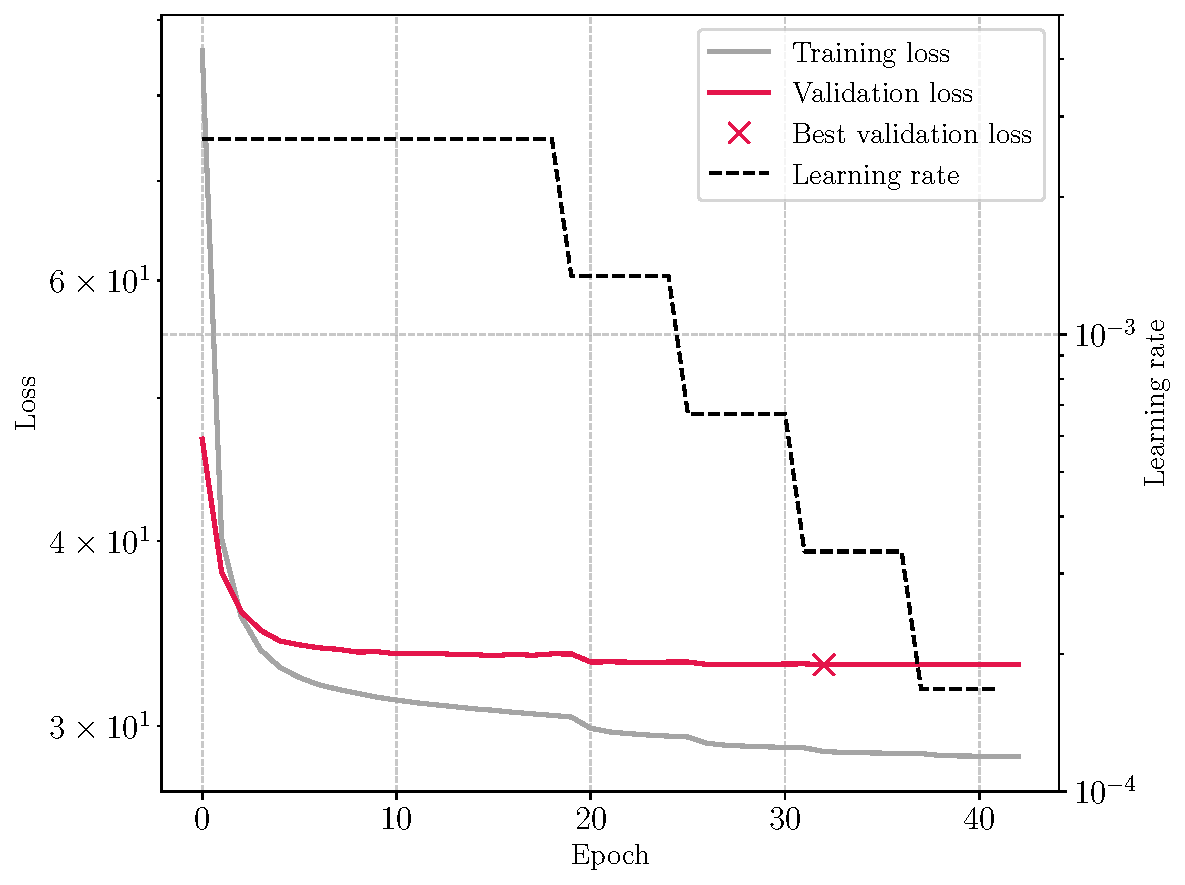
\includegraphics[width=\textwidth]{../fig/gnn/mgnn_pcseg1_simple_loss.pdf}
    \caption[GNN initial training Loss]{\TODO{...}}
    \label{fig:gnn_initial_training_loss}
\end{figure}